\lstnewenvironment{Code03_04}[1][]{\lstset{basicstyle=\small\ttfamily, columns=fullflexible,framexrightmargin=+.1\textwidth, keywordstyle=\color{red}\bfseries, commentstyle=\color{blue},language=C++, basicstyle=\small, numbers=left, numberstyle=\tiny, stepnumber=1, numbersep=5pt, frame=shadowbox, #1}}{}

\chapter{Soluzione del problema numerico}

Passiamo ora a descrivere le principali classi del codice per la soluzione del problema numerico.

\begin{figure}[h!]
\centering
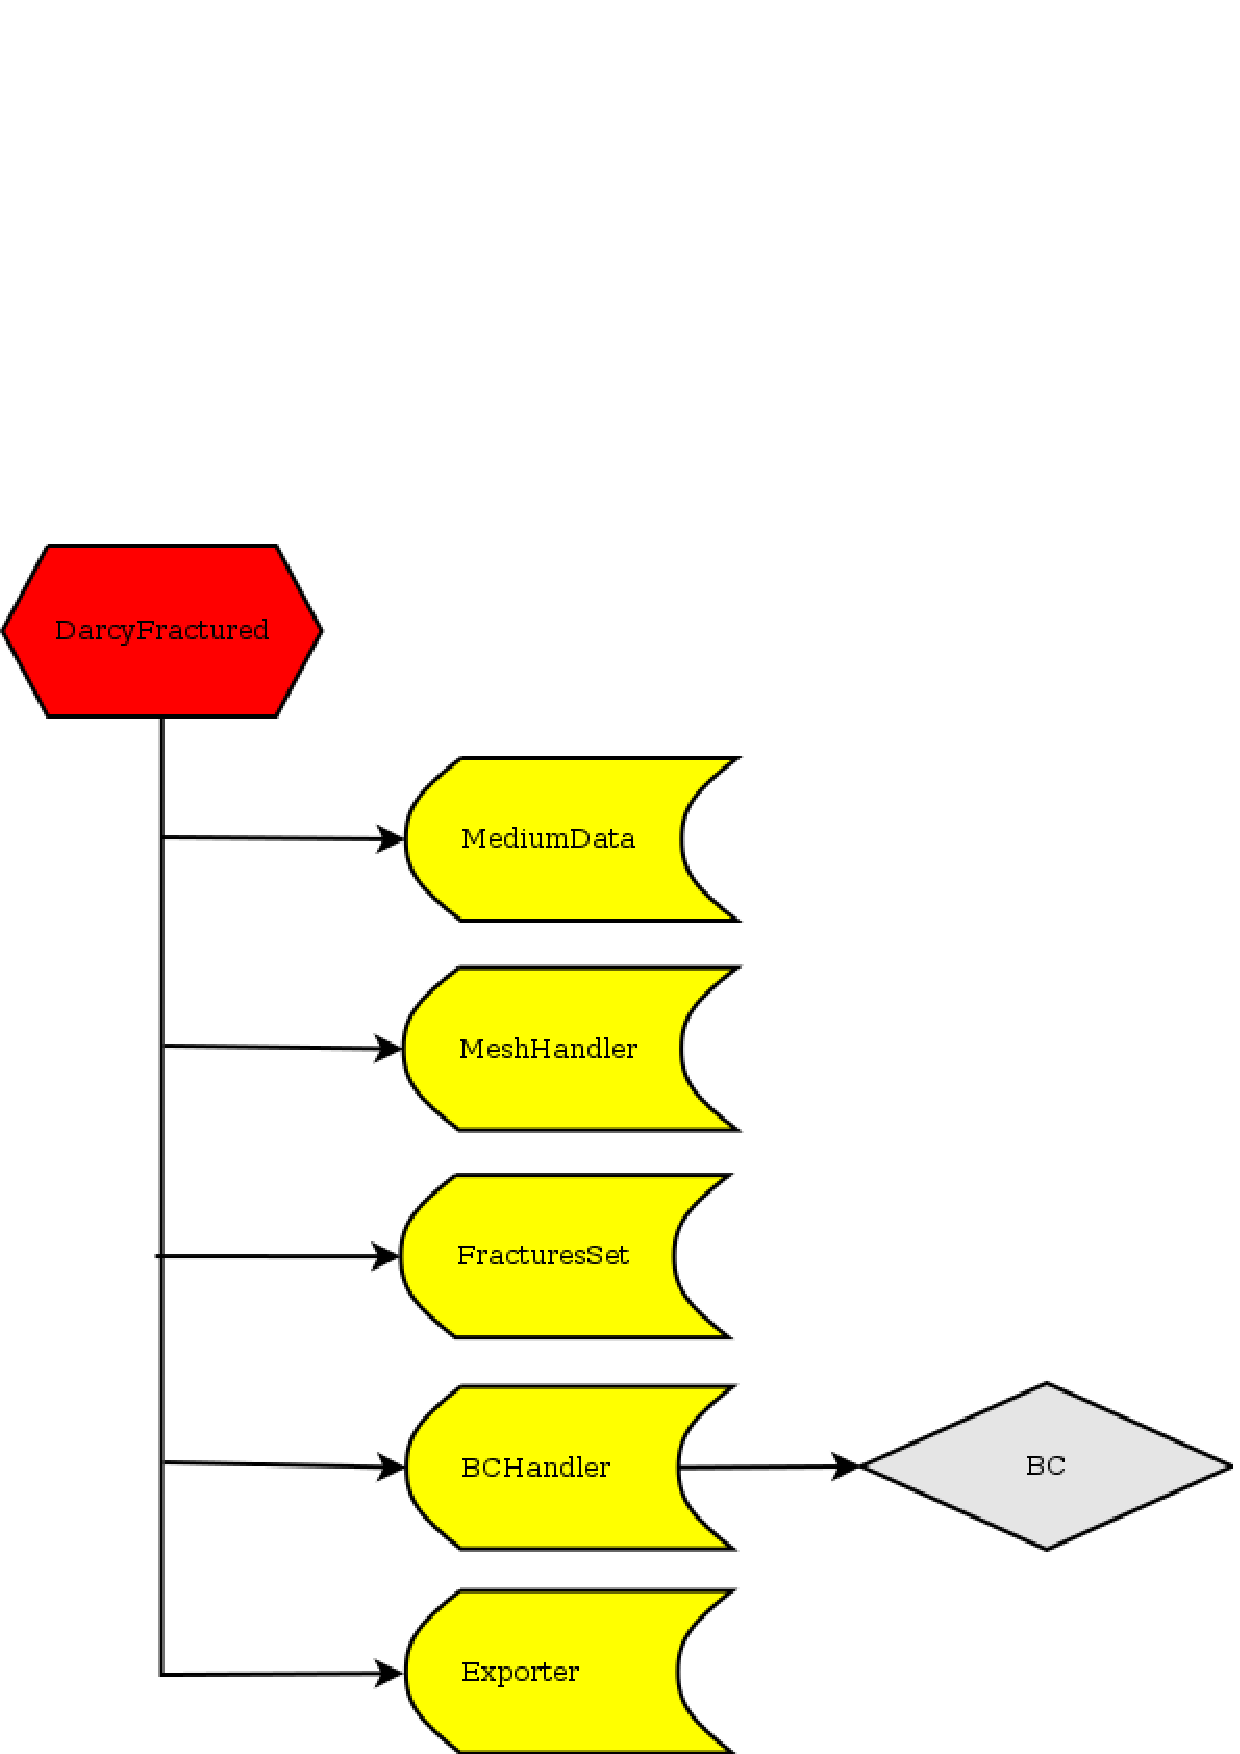
\includegraphics[scale=.59]{img/subcap3_4/DarcyFractured.pdf}
\caption{Inclusione tra le varie classi per la soluzione del problema numerico}\label{Inclusione classi DarcyFractured}
\end{figure}

\section{La Classe \texttt{DarcyFracture}}
La classe \texttt{DarcyFracture} permette di definire il problema di Darcy su ogni frattura, imporre le condizioni per le eventuali intersezioni, assemblare il sistema algebrico globale $ Ax=b $ del problema e risolverlo.\\

%Il suo costruttore richiede i seguenti parametri:
%	\begin{itemize}
%	\item \textit{Mesh:} relativa al mezzo o a una delle fratture
%	\item \textit{Stringa:} contenente il tipo di mesh di GetFem del elemento precedente
%	\item \textit{Vettore:} nullo, se la mesh fa riferimento al mezzo, contenete gli indici dei gradi di libert\`{a} degli estremi, se si sta lavorando su una frattura
%	\item \textit{ElementDimesion:} dimensione in cui stiamo lavorando ( di defaul 2 per il mezzo e 1 per le fratture)
%	\end{itemize}
\noindent I campi fondamentali della classe sono:
	\begin{enumerate}
	\item[-] \texttt{M\_globalMatrix}, matrice sparsa che rappresenta la matrice globale del sistema;
	\item[-] \texttt{M\_globalRightHandSide}, vettore del termine noto;
	\item[-] \texttt{M\_velocityAndPressure}, vettore soluzione delle velocit\'{a} e della pressione.
	\end{enumerate} 

\begin{Code03_04}[caption={Classe \texttt{DarcyFracture}}]
class DarcyFractured
{
 public:
    DarcyFractured ( const MediumDataPtr_Type& medium,
                     const MeshHandlerPtr_Type& mesh,
                     const BCHandlerPtr_Type& bcHandler,
                     const FracturesSetPtr_Type& fractures,
                     const ExporterPtr_Type& exporter );
    
    void init ( );
    
    void assembly ( const GetPot& dataFile );

    void solve ( );

	[ ... ]

 private:

	[ ... ]

    sparseMatrixPtr_Type M_globalMatrix;

    scalarVectorPtr_Type M_globalRightHandSide;

    scalarVectorPtr_Type M_velocityAndPressure;

    [ ... ]
};
\end{Code03_04}

Le funzioni fondamentali della classe sono il metodo \texttt{assembly ()} e il metodo \texttt{solve ()}. \\
\noindent Il metodo \texttt{assembly ()} crea la matrice globale $A$ e il termine noto di destra, utilizzando le funzioni della classe \texttt{XFEMOperators}. 
La matrice globale del sistema ha una struttura a blocchi, dove ad ogni frattura corrisponde un blocco derivante dal sistema \ref{sistemaAlgebrico}. Una volta definite le forme bilineari e i blocchi della matrice corrispondenti alle singole fratture, vanno imposte le condizioni d'interfaccia nel caso di eventuali intersezioni.\\
\noindent Nel caso di un \textit{Cross} si impongono le condizioni di interfaccia in maniera debole tramite le matrici $E_{2}$ e $E_{3}$, che impongono il salto di velocità nell'intersezione.\\
\noindent Nel caso di una \textit{Bifurcation} si impongono in maniera forte le condizioni di interfaccia \ref{condizioni d'interfaccia}.\\
Ipotizzando di essere in una situazione dove tre fratture hanno un intersezione di tipo \textit{Bifurcation} e una di queste si incontra con una quarta creando un intersezione di tipo \textit{Cross}, la matrice globale avrà il seguente volto:\\
%---->DA SISTEMAREEEEE <----------------- 
 \begin{center}
  $ \left[ \begin{matrix}
 			A_{0} &  B_{0} & 0 & 0 & 0 & 0 & 0 & 0 & 0 & 0\\ 
 			B_{0}^{T} & 0 & 0 & 0 & 0 & 0 & 0 & 0 & 0 & 0\\
 			0 & 0 & A_{1} &  B_{1} & 0 & 0 & 0 & 0 & 0 & 0 \\ 
		 	0 & 0 & B_{1}^{T} & 0 & 0 & 0 & 0 & 0 & 0 & 0 \\
		 	0 & 0 & 0 & 0 & A_{2} &  B_{2} & 0 & 0 & E_{2} & 0\\ 
		 	0 & 0 & 0 & 0 & B_{2}^{T} & 0 & 0 & 0 & 0 & 0\\
		 	0 & 0 & 0 & 0 & 0 & 0 & A_{3} &  B_{3} & 0 & E_{3} \\ 
 			0 & 0 & 0 & 0 & 0 & 0 & B_{3}^{T} & 0 & 0 & 0\\
 			0 & 0 & 0 & 0 & 0 & 0 & 0 & 0 & App_{0} & App_{1} \\
 			0 & 0 & 0 & 0 & E_{2}^{T} & 0 & E_{3}^{T} & 0 & 0 & 0\\
 			\end{matrix}.\right] $ 
  \end{center}
Infine il metodo \texttt{solve ()} risolve il problema e esporta i risultati ottenuti in formato \emph{vtk} per entrambe le incognite.\\

%\section{Class \texttt{XFEMOperetors}}
%Ogni frattura ha associata la matrice:
%\begin{center} 
% $ \left[ \begin{matrix}
% 	A11 &  A12 \\ 
% 	A12^{T} & 0
% \end{matrix}\right] $
%\end{center} 
%
%La classe \texttt{XFEMOperators} implementa le funzioni che ci permettono di calcolare questi blocchi.
%Le sue funzioni principali sono le seguenti:
%
%\begin{Code03_03}[caption={Funzioni per assemblare la matrice globale}]
%//Costruisce  A11 = Aij = a(\phi_j, \phi_i)
%void darcy_A11F ( sparseMatrixPtr_Type& M,
%                  const FractureHandlerPtr_Type& fracture,
%                  const scalar_type& gammaU,
%                  const scalarVector_Type& invKTangentialInterpolated,
%                  const sizeVector_Type &ExtBoundary,
%                  const size_type& uncutRegionFlag );
%
%// Aggiorna A11 nel caso intersezione" Cross "
%void darcy_A11F_Cross ( sparseMatrixPtr_Type& M,
%					    const FractureHandlerPtr_Type& fracture,
%					    const scalarVector_Type& invKTangentialInterpolated,
%					    const FractureHandlerPtr_Type& otherFracture,
%					    const size_type& cutRegionFlag );
%
%//Costruisce A12 = Bij = b(\phi_j, \omega_i)
%void darcy_A12F ( sparseMatrixPtr_Type& M,
%                  const FractureHandlerPtr_Type& fracture,
%                  const size_type& uncutRegionFlag );
%
%//Aggiorna A12 = Bij = b(\phi_j, \omega_i) nel caso di intersezione " Cross "
%void darcy_A12F_Cross ( sparseMatrixPtr_Type& M,
%                  	    const FractureHandlerPtr_Type& fracture,
%                  	    const FractureHandlerPtr_Type& otherFracture,
%                  	    const size_type& cutRegionFlag );
%\end{Code03_03}
%
%Altre importanti funzioni sono quelle che ci permetto di costruire il termine noto e son sempre contenute in questa classe.
